\documentclass[tikz,border=5mm]{standalone}
\usepackage[utf8]{vietnam}
\usepackage{amsmath,amssymb}
\usepackage{tikz}
\usepackage{pgfplots}
\pgfplotsset{compat=1.18}
\usetikzlibrary{calc,arrows.meta}

\begin{document}

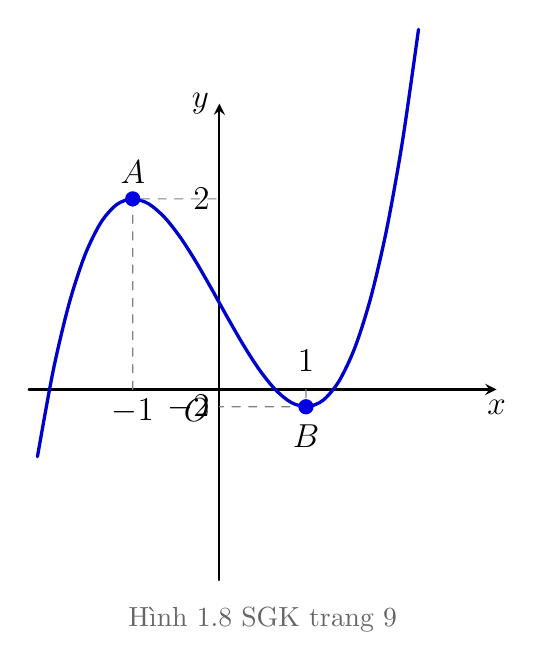
\begin{tikzpicture}[>=stealth,line join=round,line cap=round,scale=1.1,font=\large]
  \draw[->, thick] (-2.2,0) -- (3.2,0) node[below] {$x$};
  \draw[->, thick] (0,-2.2) -- (0,3.3) node[left] {$y$};
  \node[below left] at (0,0) {$O$};

  \draw[very thick, blue!80!black, smooth, domain=-2.1:2.3] plot (\x, {0.6*((\x)^3 - 3*(\x)) + 1});

  % Diem A(-1; 2) va B(1; -2)
  \coordinate (A) at (-1, 2.2);
  \draw[dashed, gray] (-1,0) node[below, text=black] {$-1$} -- (A) -- (0,2.2) node[left, text=black] {$2$};
  \fill[blue!90!black] (A) circle (2.5pt) node[above=2pt, text=black] {$A$};

  \coordinate (B) at (1, -0.2);
  \draw[dashed, gray] (1,0) node[above=3pt, text=black] {$1$} -- (B) -- (0,-0.2) node[left, text=black] {$-2$};
  \fill[blue!90!black] (B) circle (2.5pt) node[below=3pt, text=black] {$B$};
  
  \node[below, font=\normalsize, text=gray!80!black] at (0.5, -2.4) {Hình 1.8 SGK trang 9};
\end{tikzpicture}

\end{document}
